\section{Сценарии}

\subsection{Сценарий 1. Simple Speaker Listener}  \label{exp-ssl}

Сценарий \textit{Simple Speaker Listener} воспроизводится и тестируется с использованием алгоритма MADDPG \cite{lowe2017multiagent}.

Сценарий упоминается в разделе \hyperref[intro:ssl]{Вводная глава: Сценарий 1. Simple Speaker Listener}. В этом сценарии два агента имеют разные пространства действий и наблюдений. Наблюдение \textit{говоруна} $o_s$ - это цвет цели, обозначенный 3- канальным вектором $d \in \mathbb{R}^3$. Наблюдение \textit{слушателя} $o_l$ – это вектор конкатенации его собственной скорости $\upsilon \in \mathbb{R}^2$ его расстояния до трёх ориентиров $p = [p_1, p_2, p_3], p_i \in \mathbb{R}^2$ и сигнал, произнесённый \textit{говоруном} на предыдущем временном шаге. Это:

\begin{equation}
    \begin{multlined}
        o_s = [d] \\
        o_l = [\upsilon, p, c]
    \end{multlined}
\end{equation}

Коммуникационное действие \textit{говоруна} обозначается «one-hot encoding» вектором $[1; 0; 0]$ или $[0; 1; 0]$ или $[0; 0; 1]$, для обозначения трёх ориентиров соответственно.
Физическое действие \textit{u} слушателя - это 5-канальный вектор, каждый из которых представляет одно направление движения (вверх, вниз, влево, вправо или без движения). Наблюдения и действия \textit{говоруна} и \textit{слушателя} и их взаимосвязь показаны на рисунке \firef{fig:ch4-ssl}.

\begin{figure}[ht!]
    \center
    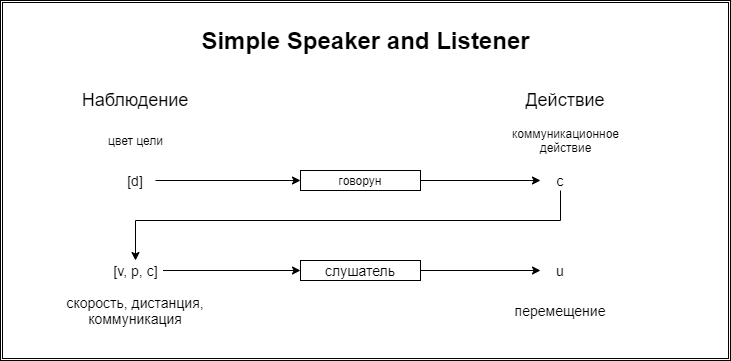
\includegraphics [scale=0.60] {my_folder/images/ch4/simple_speaker_listener.png}
    \caption{\textit{Говорун} наблюдает цвет целевого ориентира \textit{d} и издаёт коммуникационое действие, которое будет получено \textit{слушателем}. \textit{Слушатель} производит физическое движение}
    \label{fig:ch4-ssl}
\end{figure}

Два агента имеют общую награду \textit{r}, которая является отрицательным \textit{евклидовым расстоянием} между \textit{слушателем} и его целью. Проблема, которую необходимо решить в этом сценарии, заключается в поиске оптимальных политик для \textit{говоруна} и \textit{слушателя}, чтобы максимизировать ожидаемую награду, то есть $\max_{\pi}R(\pi)$, где

\begin{equation}
    \begin{multlined}
        R(\pi) = \mathbb{E}[\sum_{t=0}^{T}r(s_t, a_t)]
    \end{multlined}
\end{equation}

Во время обучения \textit{говорун} учится различать три ориентира и передавать целевой ориентир \textit{слушателю}. И \textit{слушатель} должен изучить закодированные высказывания, говоруна, и перейти к правильной цели.

Архитектура \textit{актор}-сети \textit{говоруна} аналогична архитектуре \textit{слушателя}, каждый из которых содержит два полносвязанных слоя с 64 нейронами и использует функцию активации \textit{relu}. Однако их выходные слои различаются с точки зрения количества единиц. Сети \textit{критиков} имеют структуру, аналогичную сетям \textit{акторов}, за исключением того, что они выдают скалярное Q-значение.

На этом сценарии было произведено измерение консистентности коммуникационных действий для алгоритмов DDPG и MADDPG.

\subsection{Сценарий 2. Simple Reference} \label{exp-sr}

\textit{Simple Reference} - это более сложный сценарий, который расширяет \textit{Simple Speaker Listener}.

Проблема, которую необходимо решить в этом сценарии, была изложена в разделе \hyperref[intro-sr]{Вводная глава: Сценарий 2. Simple Reference}. На \firef{fig-intro-sr} показан сценарий игры и поведение агентов при использовании оптимальных политик. В этом сценарии оба агента одновременно выступают и \textit{слушателями}, и \textit{говорунами}, что означает, что они оба выполняют как физические, так и коммуникационные действия. Высказывание каждого агента на одном шаге наблюдается другим агентом на следующем шаге, как показано на \firef{fig:exp-sr}. % TODO: сверить имя главы

Каждый агент наблюдает скорость , расстояние до ориентиров , цвет цели другого агента и высказывание другого агента. Действие каждого агента состоит из двух под-действий: физического движения $u$ и коммуникационного действия $c$.

Наблюдение и действие:

\begin{equation}
    \begin{multlined}
        o_i = [\upsilon, p, d, c] \\
        a_i = [u, c]
    \end{multlined}
\end{equation}


Это показано на \firef{fig:exp-sr}.

Наградой каждого агента является среднее значение отрицательных \textit{евклидовых расстояний} от агентов до их целей. Таким образом, оцениваются как физические, так и коммуникационные действия агентов. Предположим, что $r_0$ - это отрицательное евклидово расстояние от агента 0 до его цели, а $r_1$ - это расстояние от агента 1 до его цели. Окончательная награда для каждого агента:

\begin{equation}
    \begin{multlined}
        r = \frac{r_0 + r_1}{2}
    \end{multlined}
\end{equation}

$r_0$ используется для оценки физического движения $u_0$ агента 0 и коммуникационного действия $c_1$ агента 1. Тоже относится и к $r_1$ - он используется для оценки физического движения $u_1$ агента 1 и высказывания $c_0$ агента 0. Это показано на рисунке.

Архитектура нейронных сетей \textit{актора-критика} двух агентов в этом сценарии аналогична архитектуре в предыдущем сценарии.

\begin{figure}[ht!]
    \center
    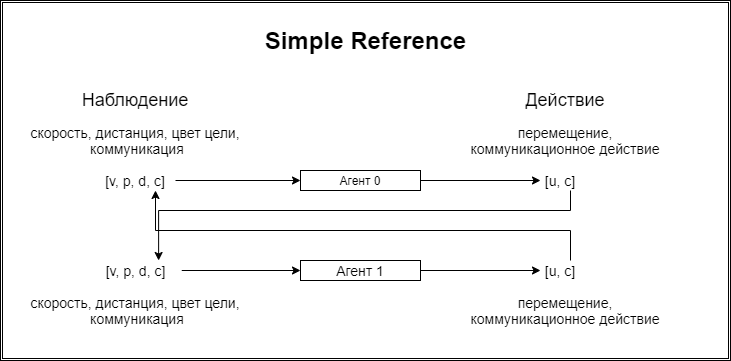
\includegraphics [scale=0.60] {my_folder/images/ch4/simple_reference.png}
    \caption{Каждый агент наблюдает целевой ориентир другого и производят коммуникационное действие, которое будет получено другим агентом на следующем шаге}
    \label{fig:exp-sr}
\end{figure}

В этом сценарии был поставлен эксперимент с \textit{декомпозированным вознаграждением}, а также эксперимент с \textit{общим мозгом}

Так же на этом сценарии производилось измерение консистентности коммуникационных действий.

\subsection{Сценарий 3. Simple World Communication} \label{exp-swc}

Кратко, этот сценарий был описан в разделе \hyperref[intro-swc]{Вводная глава: Сценарий 3. Simple World Communication}. На \firef{fig:swc} показан сценарий игры и поведение агентов при использовании оптимальных политик. В этом сценарии \textit{лидер} выступает \textit{говоруном}, остальные преследователи – \textit{слушателями}. И те и другие перемещаются, в погоне за хорошими агентами. \textit{Лидер} одновременно выступают и слушателями, и говоруном. Высказывание лидера на одном шаге наблюдается другими преследователями на следующем шаге, как показано на \firef{fig:exp-swc}.

\textit{Хорошие агенты}, просто, наблюдают \textit{еду} и \textit{преследователей} и перемещаются.

\begin{figure}[ht!]
    \center
    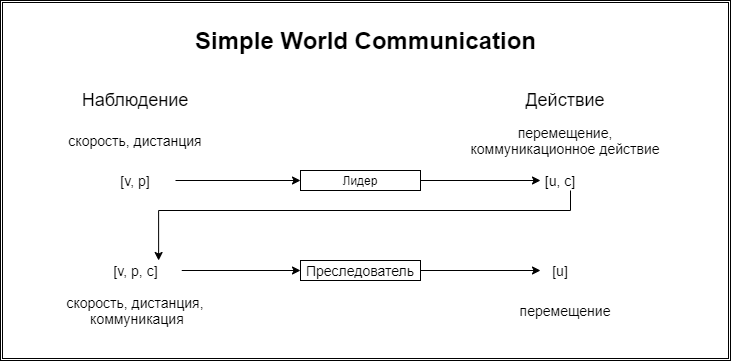
\includegraphics [scale=0.60] {my_folder/images/ch4/simple_world_communication.png}
    \caption{Лидер видит то, чего, возможно, не видят другие преследователи и производят коммуникационное действие, которое будет получено ими на следующем шаге}
    \label{fig:exp-swc}
\end{figure}

Каждый преследователь наблюдает скорость $\upsilon \in \mathbb{R}^2$, расстояние до жертв $p = [p_1, p_2, p_3], p_i \in \mathbb{R}^2$ и высказывание лидера. Лидер наблюдает тоже самое, кроме высказывания. Действие лидера состоит из двух под-действий: физического движения $u$ и коммуникационного действия $c$. Действие преследователя – только из физического движения $u$.
Наблюдение и действие лидера:

\begin{equation}
    \begin{multlined}
        o_i = [\upsilon, p] \\
        a_i = [u, c]
    \end{multlined}
\end{equation}

Наблюдение и действие преследователя:
\begin{equation}
    \begin{multlined}
        o_i = [\upsilon, p, c] \\
        a_i = [u]
    \end{multlined}
\end{equation}

Это показано на рисунке \firef{fig:exp-swc}.

Наградой каждого преследователя является отрицательное евклидовое расстояние до ближайшего агента.

Во время обучения лидер учится, как закодировать положение жертвы, чтобы передать его преследователю. И преследователь должен изучить закодированные высказывания, лидера, и двигаться к жертве.

Архитектура нейронных сетей в этом сценарии аналогична архитектуре в предыдущем сценарии.

На этом сценарии производилось измерение консистентности коммуникационных действий.

\subsection{Сценарий 4: Simple Tag} \label{exp-st}

Кратко, этот сценарий был описан в разделе \hyperref[intro-st]{Вводная глава: Сценарий 4. Simple Tag}. На \firef{fig:st} показан сценарий игры и поведение агентов при использовании оптимальных политик. В этом сценарии нет общения между агентами, но пространства наблюдения и действий всех преследователей совпадают, это позволяет применить к нему метод \textit{обучения с одним мозгом}. В этом сценарии все агенты наблюдают друг друга и перемещаются по игровому полю.

Каждый преследователь наблюдает скорость $\upsilon \in \mathbb{R}^2$, расстояние до жертв $p = [p_1, p_2, p_3], p_i \in \mathbb{R}^2$.

Наблюдение и действие:

\begin{equation}
    \begin{multlined}
        oi = [\upsilon, p] \\
        ai = [u]
    \end{multlined}
\end{equation}

Наградой каждого преследователя является отрицательное \textit{евклидовое расстояние} до ближайшего агента.

Во время обучения преследователи учатся догонять жертву, а жертва – убегать.

Архитектура нейронных сетей в этом сценарии аналогична архитектуре в предыдущем сценарии.

На этом сценарии ставился эксперимент с \textit{одним мозгом}.

\newpage

\section{Сетевая архитектура} \label{network-architecture}

В таблице \taref{tab-algs-application} показано применение различных сетевых архитектур к различным игровым сценариям.

\begin{table}[t!]
	\centering\small
	\caption{Подходящие сетевые архитектуры для разных игровых сценариев}
	\label{tab-algs-application}
	\begin{tabular}{|l|l|l|l|l|l|}
		\hline
		& MADDPG & MADDPG с одним мозгом & Декомпозированная награда \\
		\hline
		Speaker Listener    & v      & ---                     & ---                         \\ \hline
		Simple Reference    & v      & v                     & v                         \\ \hline
		World Communication & v      & ---                     & v                         \\ \hline
		Simple Tag          & v      & v                     & ---                         \\ \hline
	\end{tabular}
	\normalsize% возвращаем шрифт к нормальному
\end{table}

Такие сценарии, как \textit{Simple Speaker Listener} с двумя агентами, разделяющими глобальное вознаграждение, но обладающими разными наблюдениями и пространствами действий, могут использовать только стандартный MADDPG. Поскольку агенты функционируют по-разному, им необходимо искать различные оптимальные политики для своих ролей в игре.

Такие сценарии, как \textit{Simple Reference}, где два агента совместно получают глобальное вознаграждение, имеют одно и то же пространство действий и пространство наблюдений могут работать со стандартным MADDPG, а также эти сценарии могут использовать \textit{общий мозг}, или \textit{декомпозированную награду}.

Наиболее эффективной архитектурой являются использование сети с \textit{общим мозгом}, поскольку при этом обучается меньшее количество сетей. Это значительно повышает эффективность обучения игровых сценариев, которые можно адаптировать к сетям с \textit{общим мозгом}.

В сценарии \textit{Simple Tag} агенты из одной «команды» так же имеют одинаковые пространства наблюдений и действий. Здесь был применён отдельный набор \textit{акторов-критиков} для \textit{преследователей} и отдельный - для \textit{жертв}. Общение в этом сценарии отсутствует, поэтому \textit{декомпозированная награда} здесь не применима. Этот сценарий был выбран для сравнения стандартного MADDPG и MADDPG с \textit{одним мозгом}.

В экспериментах со сценариями, в которых агенты общаются между собой (см. \taref{tab-communicational-scenarious}), производилось измерение консистентности коммуникационных действий.

\begin{table}[t!]
	\centering\small
	\caption{Наличие действий общения в сценариях}
	\label{tab-communicational-scenarious}
	\begin{tabular}{|l|l|l|l|l|l|}
		\hline
		& Предполагает общение агентов\\
		\hline
		Speaker Listener    & v \\ 
		\hline
		Simple Reference    & v \\ 
		\hline
		World Communication & v \\ 
		\hline
		Simple Tag          & --- \\ 
		\hline
	\end{tabular}
	\normalsize% возвращаем шрифт к нормальному
\end{table}

Сценарии, в которых одни и те же агенты и перемещаются и говорят, подходят для применения \textit{декомпозированой награды}. Simple Listener не подходит, т.к. один агент только перемещается, а другой только говорит, а в Simple Tag нет действий общения.

Таким образом, для ответа на \hyperref[intro-questions]{вопросы исследования} ставились эксперименты, показывающие общение агентов между собой, а так же эксперименты, показывающие эфективность некоторых модификаций алгоритма, направленных на ускорение обучения. Исходя из этого и выбирались сценарии для экспериментов данной работы.

\newpage
